\chapter{Water Hardness Detection in Building Water Supply}
\label{chap:water}

\section{Introduction}

Domestic and Industrial water supply contain dissolved minerals of varying concentration.
 The "hardness" of water \cite{WhatIsWaterHardness} is used to refer to a certain subset of dissolved minerals, specifically Calcium and Magnesium.
 In domestic water supply, the dissolved minerals contributing to hardness affect the longevity of appliances \cite{SoftenedWaterBenefitsStudy} while simulatenously increasing health risks to the occupants \cite{PotentialHealthImpactsOfHardWater} \cite{WaterHardnessOnCardiovascularDisease}.
 In industrial water supply, especially medical research labs, mandate extremely low hardness levels.
 Consequently, water softening solutions are sought to minimize the ill effects of water hardness.

A typical solution to the water hardness levels is to install water softeners in the consuming units (residential or industrial units).
 Water Softeners are a primary source of Sodium and Chloride ion pollution in fresh water sources.
 The pollution arises as a result of softener regeneration, which produces effluent water with exteremely high mineral concentration (extremely high water hardness).
 This effluent finds its way into water treatments facilities which face challenges in removing the dissolved minerals.

The regeneration process is triggered in the water softeners based on a threshold on the aggregate water flow through the softener since the last regeneration.
 This is referred to as the "reserve capacity algorithm".
 Since the regeneration process is blind to the actual hardness in the water, there are three possible cases:

\begin{enumerate}
\item \emph{Case 1:} The regeneration happens \textbf{after} the softener has depleted its capacity, allowing hard water to reach the consumers and appliances.
 This is undesirable.
\item \emph{Case 2:} The regeneration happens \textbf{before} the softener has depleted its capacity, resulting in higher regeneration frequency and increased softener effluent discharge to water treatment facilities.
 This is undesirable.
\item \emph{Case 3:} The regeneration happens at the \textbf{exact} time when the softener is close to depletion, achieving balance between frequent regenerations and hard water mitigation.
\end{enumerate}

Case 3 does not occur in commercial water softeners since the softeners are programmed pessimistically and favor frequent regenerations (Case 2) to minimize the risk of hard water reaching the consumer (Case 1).
 As a solution to this pessimism, the AWESOME system \cite{AWESOME} provides a mechanism to control the tradeoff between Case 1 and Case 2.
 The AWESOME \cite{AWESOME} system is an example of an Edge Computing platform where the computation and intelligence is decentralized by leveraging compute power at the "edge" of connectivity (e.g. using WiFi routers in the home).
 In the case of AWESOME, Machine Learning algorithms are deployed at the edge, using edge computing resources.
 There are two key Machine Learning challenges involved in the solution.

\paragraph{Water Hardness Detection:} The hardness is measured using Calcium ion ($\CalciumIon$) sensors at the output of the water softener.
 However, the sensors do not measure a clean, trivially recognizable hardness signal.
 The measurements exhibit several "false" hardness events, where the signal shares characteristics with a true hardness event.
 We built a Support Vector Machine to distinguish between the false hardness events and the true hardness events.
 When a true hardness event occurs, it is an indication of the depleted state of the water softener.

\paragraph{Water Flow and Hardness Forecasting:} The hardness is highly dependent on the water flow patterns of the building.
 Once it is possible to distinguish between true and false hardness events from the sensor signals, predicting the flow patterns of a building would allow to forecast the exact time of the hardness event ahead of time.
 This allows flexibility in better protecting the consumers and appliances (Case 1) while minimizing effluent discharge (Case 2).





\section{Water Hardness Detection}

The objective is to devise features and learn a Support Vector Machine (SVM) that is able to distinguish between true hardness events and false hardness events in the water at the output of the water softener.


\subsection{Feature Engineering}

The following features were chosen by empirical studies as being most "informative" towards this classification task.

\begin{enumerate}
\item \emph{Measured Hardness:} This is directly calculated from the output of the Calcium ion ($\CalciumIon$).
 The sensor output is a voltage value which is converted to the corresponding hardness measurement in grains per gallon \cite{WhatIsWaterHardness}.
\item \emph{Flow Rate:} Flow rate is the average rate of flow over a 2 minute interval (can be considered as instantaneous rate of flow considering that the dynamics of the system are extremely slow).
 In this case, the "instantaneous" flow has been chosen as a feature in order to make the algorithm independent of the cumulative flow, unlike the reserve capacity algorithm.
 The reserve capacity algorithm uses the cumulative flow or the number of days since last regeneration to trigger the next regeneration \cite{NSFSoftener}.
\item \emph{Temperature:} This is chosen as a feature because the output voltage of the Calcium ion ($\CalciumIon$) sensor was found to fluctuate with the ambient temperature.
\item \emph{Derivative of the voltage output of the Calcium Ion ($\CalciumIon$) sensor:} This is used to encode some characteristics of the shape of the hardness measurement transient.
\item \emph{Temperature compensated voltage output of the Calcium Ion ($\CalciumIon$) sensor:} The relationship between the temperature and the voltage output of the sensor is highly nonliner and difficult to characterize.
 This hand engineered feature was included as a simple compensation technique for temperature effects to help the SVM improve its classification accuracy.
 This approach is similar to using kernel functions.

\end{enumerate}

The features are also described in \ref{tab:features_hard_water}. An example trace of raw hardness data is shown in Figure \ref{fig:example_trace_water_hardness}.

\subsection{Data Collection and Learning}
\label{sec:water_hardness_learning}

The data was collected from multiple installations of the AWESOME \cite{AWESOME} system over several months (with at least 2 instances of true hardness events from each installation).
 \footnote{The training was done after the appropriate pre-preprocessing using the \texttt{scikit-learn} Python library.}

SVM is a supervised learning algorithms, meaning that it requires a training phase in which input data labeled with ground truth is fed to the algorithm.
 When constructing the training sets for SVM, each feature vector with ground truth.
 I developed a web-based training tool for time-series data that allows for crowdsourced labeling.
 A screenshot of this tool is shown in in Figure \ref{fig:hardnesslabelingtool}.
 This training tool was used to directly generate data sets for SVM training.

This labeling process is subjective because the water hardness --- concentration of Calcium and Magnesium ions --- is a real number which must be converted to a binary value (0 or 1).
 So to label training data, a \textbf{training threshold} must be applied, below which water is considered to be soft (0), and above which it is considered to be hard (1).
 The threshold applied will affect the SVM's ability to distinguish between soft and hard water.
 If the training threshold is too low, the algorithm may classify all unknown inputs as hard (false positives).
 If the training threshold is too high, all hardness events may be ignored (false negatives).
 The objective is to produce training sets that will identify filtration medium depletion early (before the outgoing water has become too hard) while rejecting noise.
 This is discussed further in Section \ref{sec:water_hardness_evaluation}.

\begin{figure}[!t]
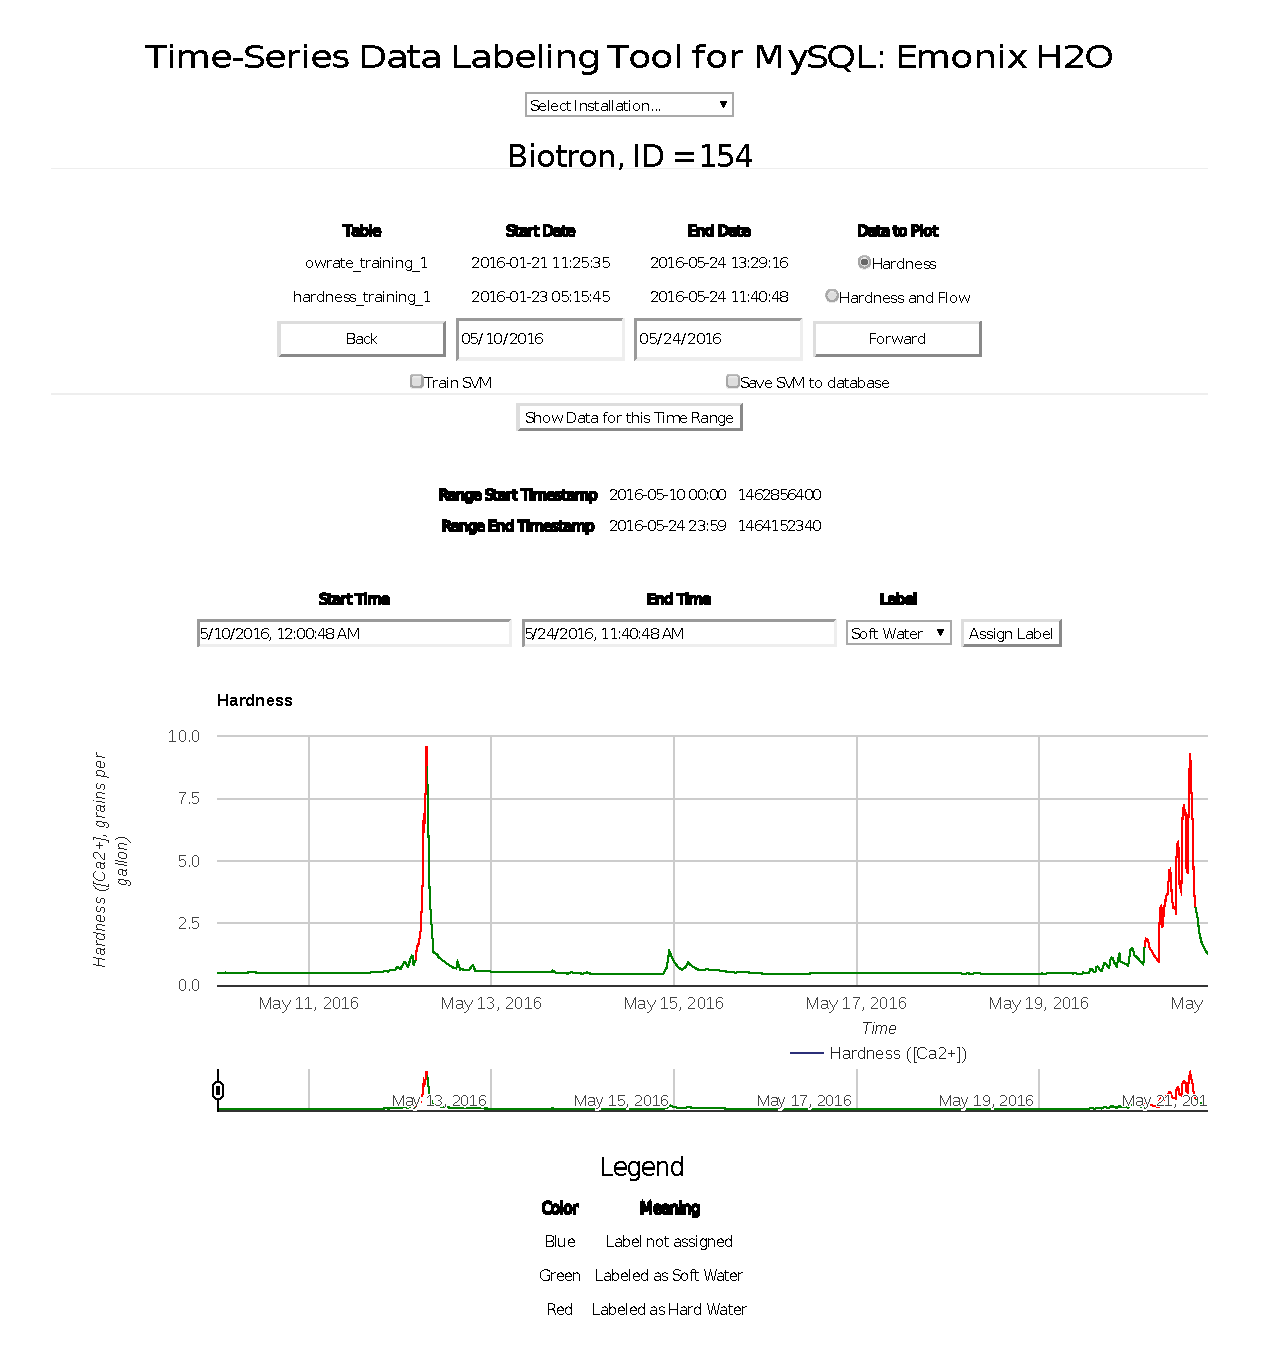
\includegraphics[width=\textwidth]{water/hardnesslabelingtool2.pdf}
\caption{Screenshot of Time-series data labeling tool developed for Water Hardness Labeling}
\label{fig:hardnesslabelingtool}
\end{figure}

\begin{table}
\centering
    \begin{tabularx}{\textwidth}{l || X || X }
    \textbf{Feature} & \textbf{Formula} & \textbf{Units} \\
    \hline
    ISE Output &  $[\CalciumIon] = e^{k (V - a)}$ & $[grains/gallon]$ \\
    Flow Rate &  $f$ & $[gal/minute]$ \\
    Temperature & $T$ & $[^\circ C]$ \\
    Derivative of ISE Output & $\frac{d [\CalciumIon]}{dt}$ & $[grains/gallon/minute]$ \\
    Normalized ISE Output & $[\CalciumIon] \left(  1 - e^{-k f / T}\right) $ & $[grains/gallon]$ \\
    \end{tabularx}
\caption{Description of hand-engineered features used to detect hard water}
\label{tab:features_hard_water}
\end{table}

\begin{figure}
\centering
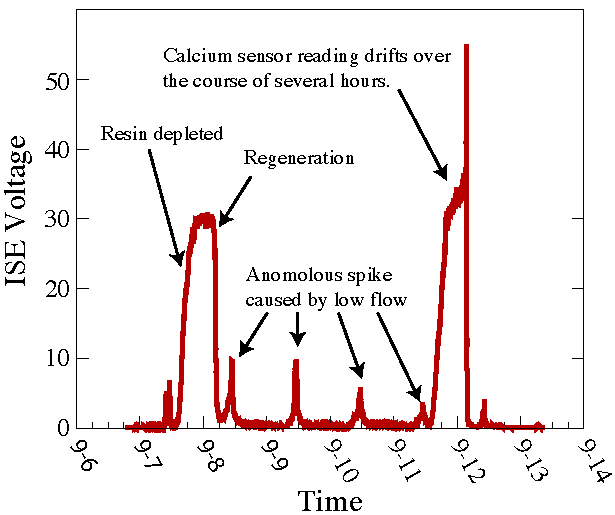
\includegraphics{water/hardness-snapshot.pdf}
\caption{Example trace of raw water hardness data showing both true and false hardness events}
\label{fig:example_trace_water_hardness}
\end{figure}

\subsection{Evaluation}
\label{sec:water_hardness_evaluation}

\begin{enumerate}
\item How quickly can the SVM identify depletion of the water softener (true hardness event)?
\item How resistant is each algorithm to anomalous sensor inputs (noise)?
\end{enumerate}

The answer to the first question will give insight that is similar to a false-negative rate.
 An important figure of merit is the amount of time it takes the system to detect water softener resin depletion.
 The earlier the detection happens, the lesser the impact of hard water on the residence or industrial facility.
 The longer it takes the SVM to detect that the resin has been depleted, the harder the water that is produced by the softener, potentially endangering building systems.

The answer to the second question will tell us the false positive rate.
 When the SVM produces a false positive, it regenerates the softener unnecessarily, wasting salt.

To identify filtration medium depletion, it will be necessary to allow the medium to deplete and start producing hard water.
 The goal is to minimize the amount of hard water that needs to be produced before the SVM can identify that the medium is depleted.
 If too much hard water is supplied to a building before initiating a regeneration, the water heater and other building systems could suffer damage.


In order to make the SVM detect hard water as early as possible, the training threshold (described in Section \ref{sec:water_hardness_learning}) is manually adjusted based on empirical performance feedback.
 The lower the training threshold is set, the earlier the SVM will be able to detect filtration medium depletion.
 Figure \ref{fig:hardnessresults} shows a plot of the average outgoing water hardness level at which the algorithm can detect medium depletion for several different training thresholds.
 The figure presentes a comparison of the hardness detection level between simple thresholding and the SVM (simple thresholding has a high false positive rate, as evident from Figure \ref{fig:example_trace_water_hardness}).
 The y-axis gives the average water hardness required for each algorithm to identify a filtration medium depletion.
 To be practical, the detection level should be below five grains per gallon because allowing the hardness to get any higher would damage building systems.


At low training thresholds, the learning algorithms tend to produce more false positives.
 Figure \ref{fig:falsepositives} shows the false positive rates on the y-axis with the algorithm on the x-axis.
 To strike a balance between minimizing false positives and minimizing the hardness detection level, it is best to train the learning algorithms to identify depletion at three grains hardness.


The receiver operating curve (ROC) shown in Figure \ref{fig:roc} shows the tradeoff between false positives and true positives for SVM and thresholding.
 On the y-axis, true positives are plotted as a function of false positives.
 The SVM performs much better than thresholding because we only need to increase the proportion of false positives to 30\% in order to achieve 90\% true positive detection.



\begin{figure}[t]
\centering
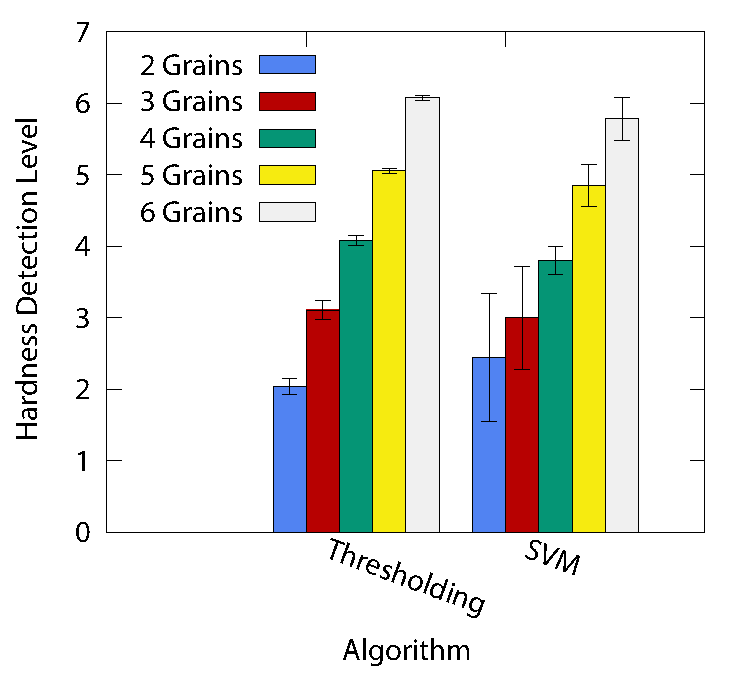
\includegraphics{water/hardnessresults.pdf}
\caption{The water hardness level of detection for five different training levels.}
\label{fig:hardnessresults}
\end{figure}


\begin{figure}[t]
\centering
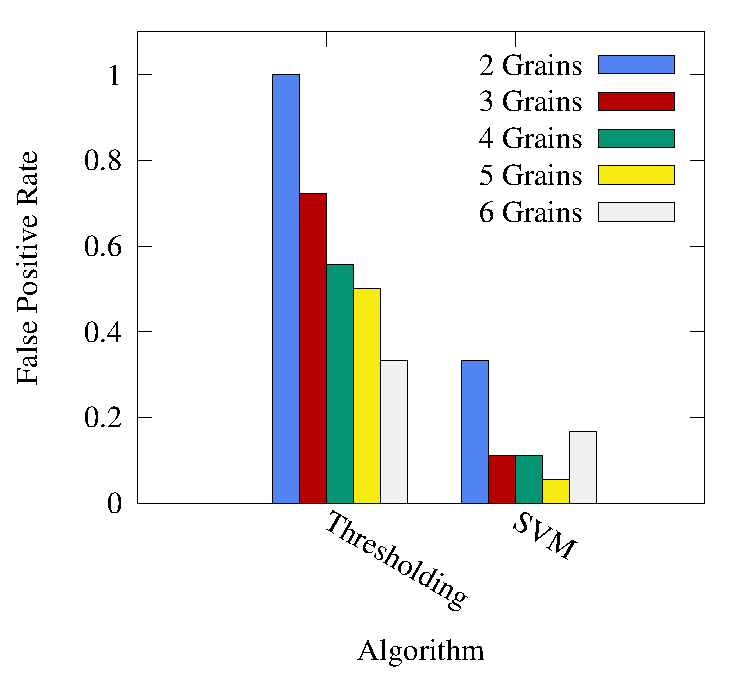
\includegraphics{water/hardnessfalsepositives.pdf}
\caption{False positive rates for the water hardness detection learning algorithm, tested with five different training thresholds.}
\label{fig:falsepositives}
\end{figure}

\begin{figure}[t]
\centering
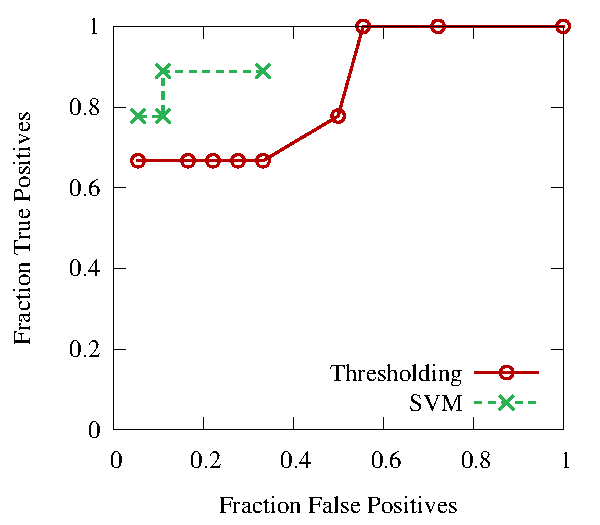
\includegraphics{water/hardnessroc.pdf}
\caption{Receiver operating curve for the water hardness detection learning algorithm.}
\label{fig:roc}
\end{figure}


\section{Water Flow and Hardness Forecasting}

The objective is to forecast water flow and water hardness at the output of the water softener based on historical patterns.
 Forecasting the water flow based on historical patterns is equivalent to modeling the water usage behaviour of a building (residential or industrial).
 Forecasting the water hardness based on historical patterns is equivalent to modeling the physics of the water softener itself and its depletion characteristics.

\subsection{Water Flow Forecasting}

A statistical analysis of water flow patterns in various buildings indicate that the flowrate function is not a stationary process over long time periods.
 \footnote{A stationary process is one whose statistical properties do not change as a function of time. In other words, $X_t$ is stationary iff $F_X (x_{t_1} ... x_{t_k}) = F_X (x_{t_{1+l}} ... x_{t_{k+l}})$}
 This finding makes sense because activities in a building will likely follow daily circadian fluctuations.
 At 4 AM, when most residents are asleep, the histogram indicates that the recorded flow rates are mostly zero.
 Flow rates increase around 8 AM when residents wake up to go to class.
 At noon, flowrates increase further because lunch is served in the building's cafeteria.
 Since the distribution of water flow rates changes during the course of the day, it is reasonable to conclude that the process is nonstationary.

Since the flowrate signal is nonstationary, the modeling approach should deal with data that has time-varying distribution.
 An autoregressive model is a commonly used tool to forecast stationary processes \cite{oppenheim2010discrete}.
 Here, the autoregressive approach is adapted to work with a nonstationary process, leveraging continuous data measurements.

The flowrate signal tends to be bursty --- it tends to be high for a short time when a fixture is turned on and low when the fixture is off.
 In large buildings, that burstiness is contributed by hundreds of fixtures, each contributing to a noisy signal with a lot of high-frequency components.
 To deal with such a large magnitude of high frequency components, an extremely high order of autoregressive model will be required, which makes the modeling infeasible.
 Instead of forecasting the raw flowrate, forecasting the cumulative flow is a reasonable compromise (equivalent to passing the flowrate signal through an integrator).
 The resulting autoregressive model will have poor accuracy in forecasting instantaneous flowrate.
 However, this cumulative flow signal is a more useful metric anyway --- the cumulative flow is the more important metric for understanding softener depletion.

The autoregressive model then predicts the cumulative flow used by the building on a minute-by-minute basis, 24 hours into the future.
 The results of the predictions made by the autoregressive model will be presented in Section \ref{sec:eval-forecasting}.

\subsection{Water Hardness Forecasting}

In addition to forecasting flow, it is also beneficial to predict water hardness readings, since it will be the better indicator of softener depletion.
 If the water softener's filtration medium will not be depleted in the near future according to predictions (i.e. water will not be hard), there is no point in regenerating the water softener.


Similar to the flow forecasting technique, a vector-state autoregressive model is used to predict future cumulative flow and hardness together.
 Unlike the flow rate signal, the hardness signal is sparse.
 Most of the hardness readings are zero or nearly zero---this is expected because when the water softener is working properly, it removes all hardness from the water.
 It is only when the water softener's filtration medium depletes that nonzero hardness is observed.
 The sparse nature of the hardness readings and the inherent nonlinearity of the hardness with respect to the cumulative water flow through the softener poses a challenge for learning linear, stationary models, such as, autoregressive models.


To account for the inherent nonlinearity so described, two operating point models are used (for low/high cumulative flow since the last regeneration).
 This is justified on the basis that the nonlinearity of the hardness measurement only manifests itself in the high flow region.
 A parallel can be drawn between this approach and the general practice of linearizing nonlinear systems near typical operating points for the design of closed-loop controllers.
 Since the hardness measurements depend on the cumulative flow through the softener since the last regeneration, in addition to the history of the hardness measurements themselves, the model can be represented in the following discrete-time state space notation ($flow(\dots)$ refers to the cumulative flow since the last regeneration):

\begin{gather}
X(k+1) = \begin{bmatrix}
A_{\text{flow-flow}} & 0_{\text{flow-hardness}} \\ 
C_{\text{hardness-flow}} & D_{\text{hardness-hardness}}
\end{bmatrix} X(k) \\
X(k) = \begin{bmatrix}
\text{flow}(k) \\
\dots \\
\text{flow}(k-20) \\
\text{hardness}(k) \\
\dots \\
\text{hardness}(k-20)
\end{bmatrix}
\end{gather}

$A_{\text{flow-flow}}$ captures the nature of the water usage by the residents of the building.
 Since this quantification is subject to rapid, unpredictable changes (nonstationarity), the forecasting model is learnt online after each regeneration cycle thereby using the most recent water usage patterns for the forecasting, eliminating bias due to historical data and addressing the nonstationary nature (resets due to regenerations).
 
 
The dependence of hardness measurements on their own history and the flow is quantified by the coefficients matrices of the mode $C_{\text{hardness-flow}}$ and $D_{\text{hardness-hardness}}$.
 The model so described is learned from recorded data for two operating regions (low/high cumulative flow since the last regeneration).
 When the actual forecasting is done, one of the models is chosen based on the flow since the last regeneration at the time of forecasting.

\subsection{Evaluating Forecasting Performance}
\label{sec:eval-forecasting}



\begin{figure*}[!th]
\centering
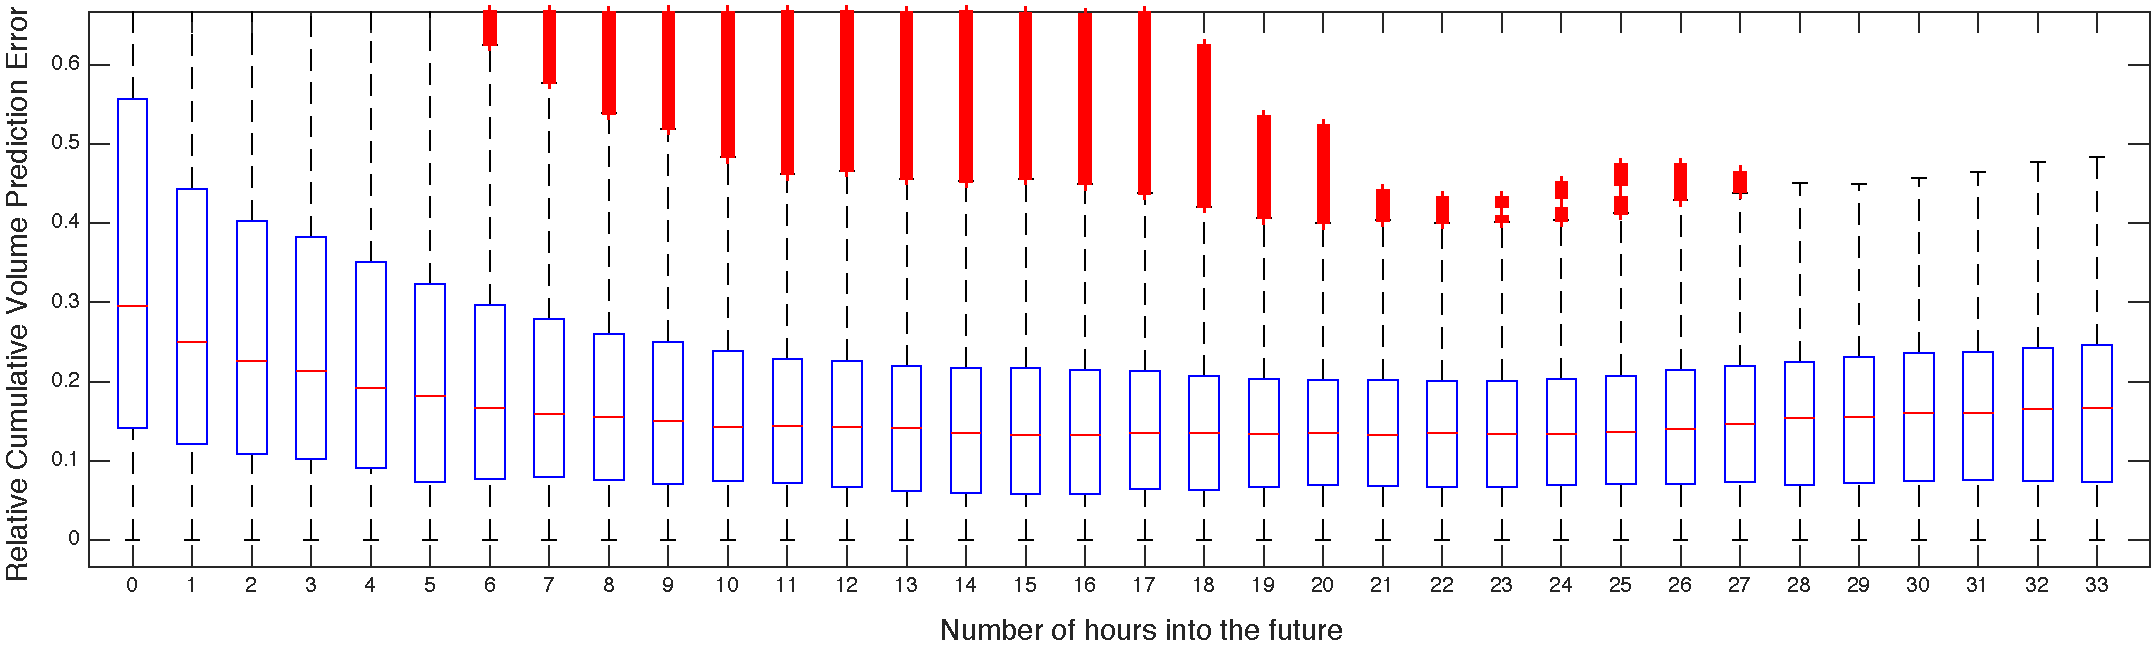
\includegraphics[width=\textwidth]{water/rel_cum_vol_pred_err.pdf}
\caption{Relative prediction error of cumulative water flow (y-axis) as a function of the forecast horizon (x-axis).}
\label{fig:cum_vol_pred_err}
\end{figure*}

\begin{figure*}[!th]
\centering
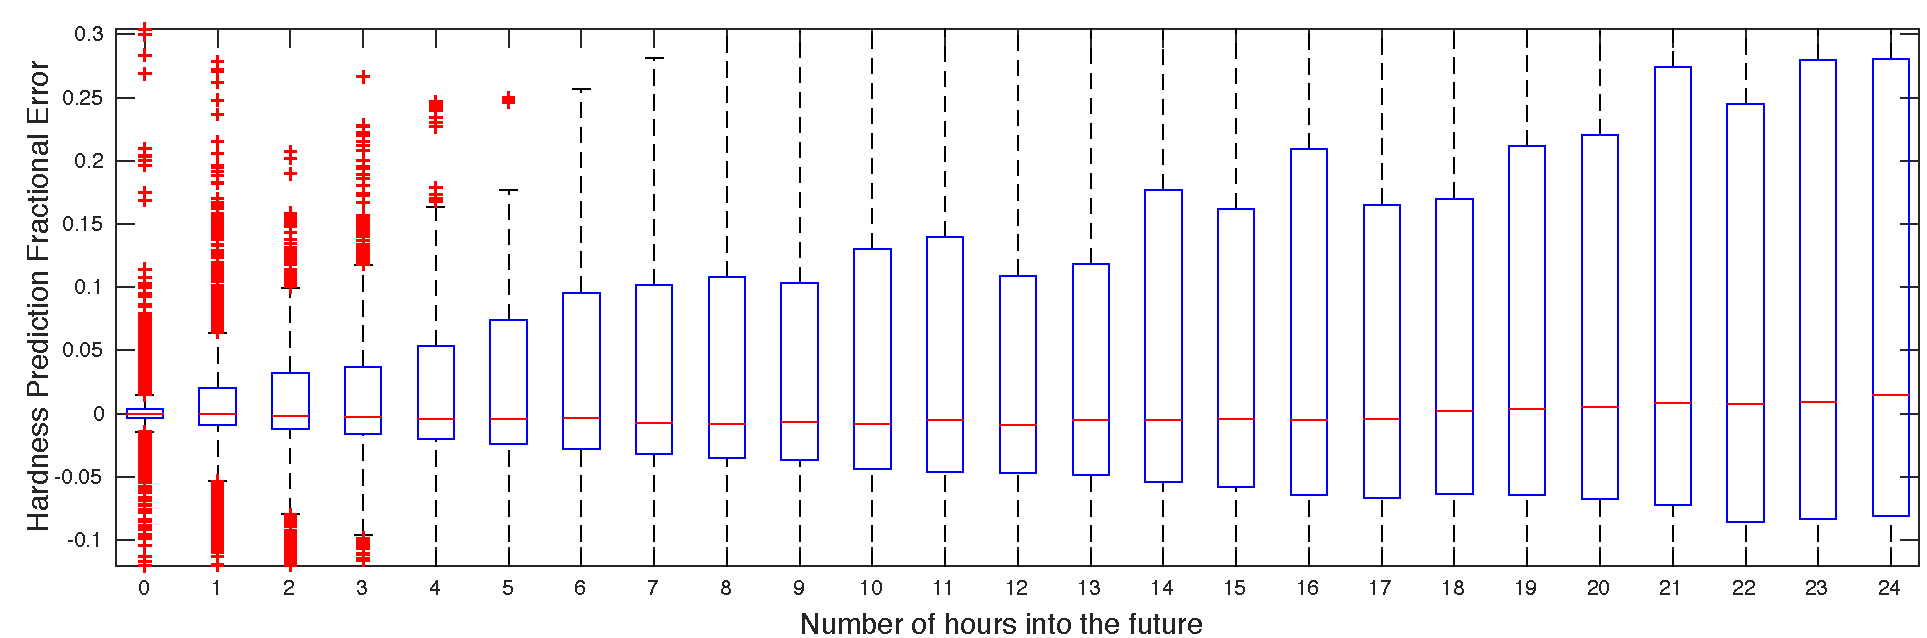
\includegraphics[width=\textwidth]{water/rel_hardness_pred_error_154.pdf}
\caption{Relative prediction error of water hardness (y-axis) as a function of the forecast horizon (x-axis).}
\label{fig:rel_hardness_pred_error_154}
\end{figure*}

\begin{figure}[!th]
\centering
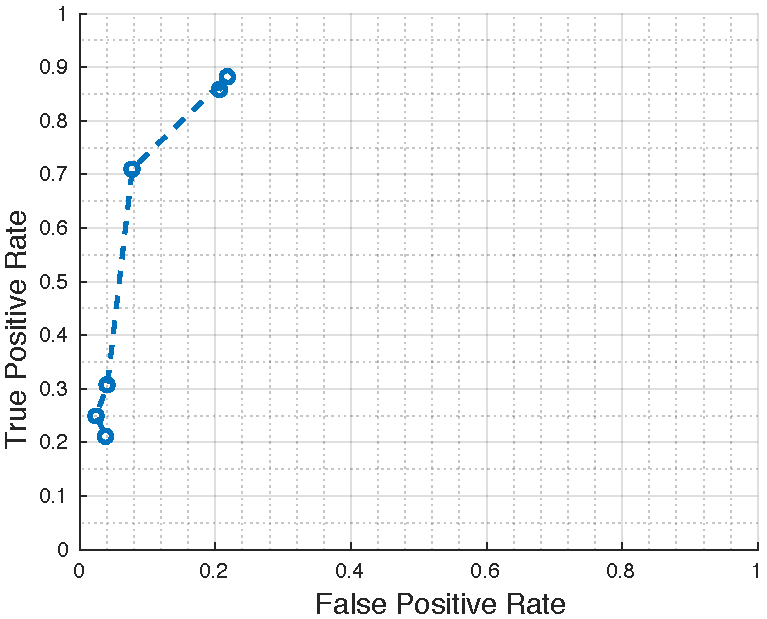
\includegraphics[width=\textwidth]{water/ROC_154.pdf}
\caption{Receiver operating characteristic for water hardness forecasting.}
\label{fig:forecastingroc}
\end{figure}

Relative prediction error is defined as

\begin{equation*}
e_{p_r}(h) = \left| \frac{p(t-h)-s(t-h)}{s(t-h)} \right|
\end{equation*}

where $h$ is the number of hours in advance the algorithm is predicting, $p(t)$ is the prediction as a function of time, and $s(t)$ is the actual measured sensor value as a function of time.
 Computations of relative prediction error for cumulative flow are shown in Figure \ref{fig:cum_vol_pred_err}.

Relative prediction error for cumulative flow is on average below 30\% and decreases for longer time horizons.
 The instantaneous flow signal tends to be very bursty---as fixtures turn on and turn off in the building, water flow starts and stops sporadically.
 If these bursts do not arrive at the exact moments that the algorithm expects them to, but instead arrive several minutes before or after, then the near-term cumulative flow error will be higher.
 As long as the bursts of flow eventually arrive, the long-term cumulative flow is low because it captures all the flow that has happened over a long period of time, and the errors in the prediction cancel each other out.

The hardness forecasting algorithm is intended to predict whether or not water samples will read hard in the next 24-hour time horizon.
 Since our water hardness sensor readings are sparse---long stretches of zero readings followed by short periods of hard water readings---the objective is to predict not only the exact value of the hardness sensor readings but also the presence or absence of hard water.
 If, during a forecasting horizon, the hardness value is not predicted accuractely but the presence or absence of a hard water event is correctly identified, then the algorithm has largely achieved its goal.

A plot of the relative errors in hardness prediction is shown in Figure \ref{fig:rel_hardness_pred_error_154}.
 On average, the relative prediction errors are close to zero for time horizons up to 24-hours in the future.
 The variance, however, increases for predictions made further into the future.


A receiver operating curve for the hardness forecasting algorithm is shown in Figure \ref{fig:forecastingroc}.
 The ROC was generated by varying the threshold at which water is classified as being hard---higher thresholds resulted in a higher false positive rate.


\section{Conclusion}


In this chapter, I describe techniques to classify water hardness based on ion concentration sensors to determine the state of water softener depletion.
 In addition, I also describe techniques to adapt commonly used autoregressive models to nonstationary, nonlinear processes with a known nonlinearity (hard resets, sudden water hardness events).
 The adaptation is required to keep the order of the autoregressive model low, which in turn keeps learning and forecasting computationally light.
